\documentclass[11pt,a4paper]{article}

\usepackage{../style/thga-db}
\usepackage{caption}
\usepackage{float}

\renewcommand{\thgaKurs}{Databases}
\renewcommand{\thgaDatum}{Summer Term 2026}
\newcommand{\authorName}{Mohamed Yassine Hachimi}
\newcommand{\projectTitle}{HandwerkerKasse -- User Guide}

\begin{document}
\thispagestyle{empty}
\thgaTitel{Term Project -- User Guide}{\projectTitle}

\begin{infobox}
\textbf{Author:} \authorName \\
\textbf{Module:} Introduction to Database Management Systems · THGA Bochum \\
\textbf{Who this guide is for:} anyone using HandwerkerKasse in their daily work -- no technical knowledge needed.
\end{infobox}

\section{What is HandwerkerKasse?}

HandwerkerKasse is a simple app for craft businesses. It helps you keep track of your customers, your jobs, the materials you use, and the invoices you send. The best part: it automatically tells you whether a job earned you money or cost you money -- no calculator needed.

\section{Getting started}

The app needs to be installed once on your computer. This is normally done for you by whoever set up the system. If you need to do it yourself, open a terminal and type:

\begin{verbatim}
sudo apt install ./handwerkerkasse.deb
\end{verbatim}

After that, you can open HandwerkerKasse like any other program: search for it in your applications menu, or type \texttt{handwerkerkasse} in a terminal.

\section{Step 1: Connect to the server}

When you open the app, you will see the connection screen shown in Figure~\ref{fig:connect}. You need to fill in two things, which you get from whoever set up your system:

\begin{itemize}
  \item \textbf{API URL} -- the address of your server. If everything runs on your own computer, this is usually \texttt{http://127.0.0.1:8000}.
  \item \textbf{X-API-Key} -- think of this like a password that lets you make changes (add customers, jobs, etc.).
\end{itemize}

Then click \textbf{Connect}. If it doesn't work, double-check the address and make sure the server is switched on.

\begin{figure}[H]
  \centering
  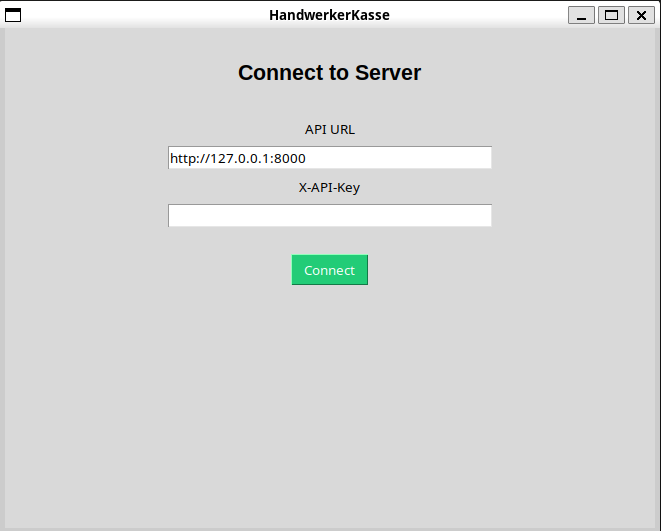
\includegraphics[width=0.6\linewidth]{09_frontend_connect-screen.png}
  \caption{The first screen you see when opening the app}
  \label{fig:connect}
\end{figure}

\section{Step 2: See all your jobs at a glance}

This is the main screen, shown in Figure~\ref{fig:overview} -- the one you will use most. It shows every job you have, and next to it how much you billed the customer, how much the materials cost, and what's left over: your profit.

\textbf{Green} means the job made you money. \textbf{Red} means it cost you more than you earned.

Use \textbf{Refresh} to update the list. Use \textbf{+ New Job} or \textbf{+ Invoice} to add something new.

\begin{figure}[H]
  \centering
  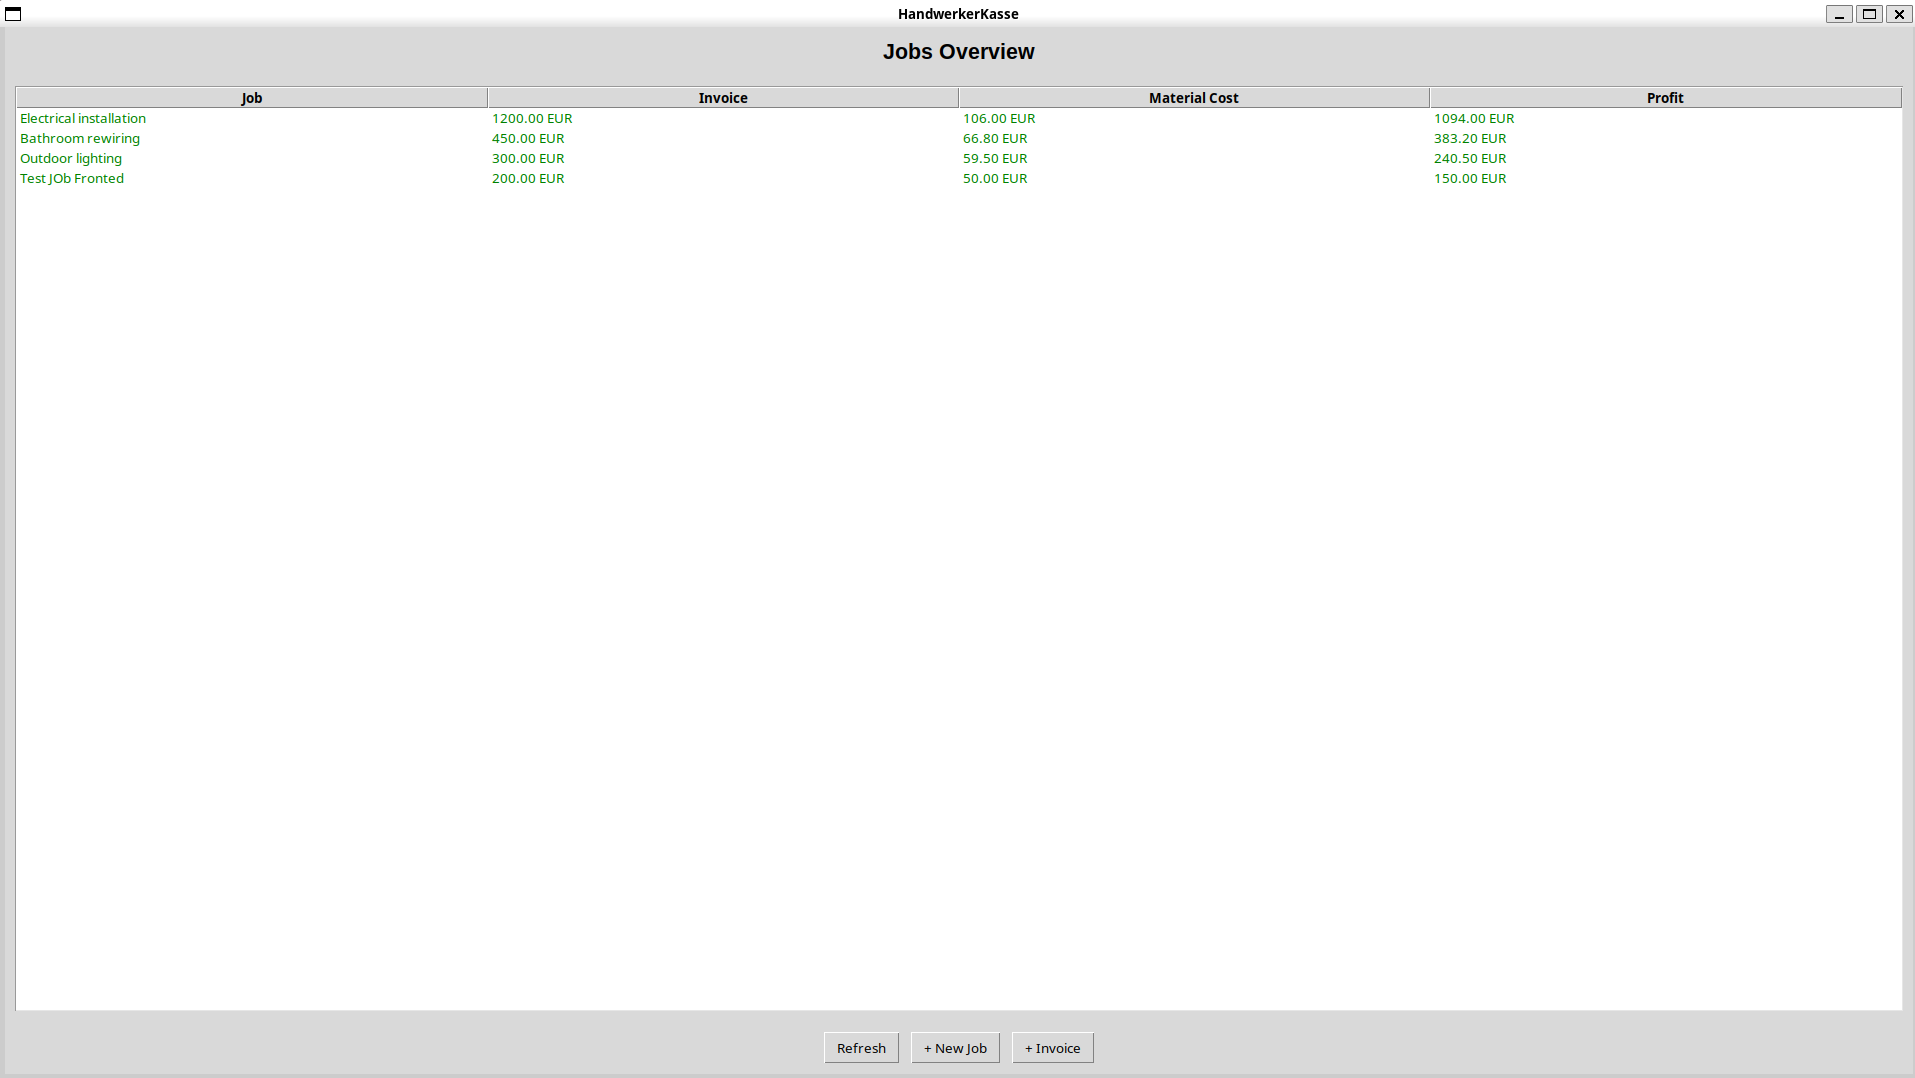
\includegraphics[width=0.75\linewidth]{10_frontend_jobs-overview.png}
  \caption{Your jobs, with profit shown automatically}
  \label{fig:overview}
\end{figure}

\section{Step 3: Add a new job}

When you start a new job, add it here, as shown in Figure~\ref{fig:jobform}:

\begin{enumerate}
  \item Type in the \textbf{customer's ID number}.
  \item Give the job a short \textbf{name}, e.g. ``New bathroom wiring''.
  \item Enter the \textbf{date}.
  \item Click \textbf{Save Job}. The app will show you the job's ID number -- keep it in mind, you'll need it in the next step.
\end{enumerate}

Once the job is saved, list the materials you used for it, at the bottom of the same screen:

\begin{enumerate}
  \item Enter the \textbf{job's ID number}.
  \item Enter the \textbf{material's ID number}.
  \item Enter \textbf{how much of it} you used.
  \item Click \textbf{Add Material}.
\end{enumerate}

Repeat this for every material you used on the job.

\begin{figure}[H]
  \centering
  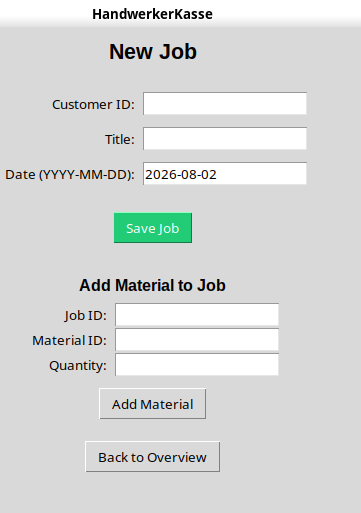
\includegraphics[width=0.75\linewidth]{11_frontend_new-job-form.png}
  \caption{Adding a job and the materials used}
  \label{fig:jobform}
\end{figure}

\section{Step 4: Send the invoice}

Once the job is done, create the invoice, as shown in Figure~\ref{fig:invoice}:

\begin{enumerate}
  \item Enter the \textbf{job's ID number}.
  \item Enter the \textbf{amount} you're billing the customer.
  \item Choose whether it's \textbf{unpaid}, \textbf{paid}, or \textbf{overdue}.
  \item Click \textbf{Create Invoice}.
\end{enumerate}

You'll be taken straight back to the overview -- and now you'll see the profit for that job, calculated automatically.

\begin{figure}[H]
  \centering
  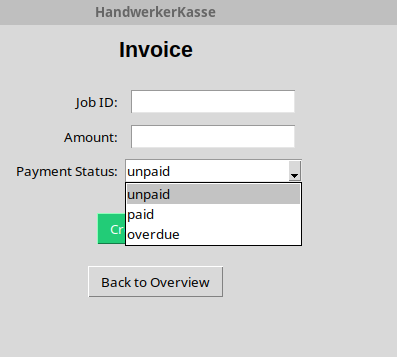
\includegraphics[width=0.75\linewidth]{12_frontend_invoice-screen.png}
  \caption{Creating an invoice}
  \label{fig:invoice}
\end{figure}

\section{How is the profit calculated?}

It's simple: what the customer paid you, minus what you spent on materials.

\begin{center}
\textit{What you earned} $-$ \textit{What the materials cost} $=$ \textit{Your profit}
\end{center}

If that number is positive, you made money on the job (shown in green). If it's negative, the materials cost more than you charged (shown in red) -- a sign to adjust your pricing next time.

\section{Something not working?}

\begin{itemize}
  \item \textbf{Can't connect at startup:} check the server address is correct, and that the server is running.
  \item \textbf{An action fails with an error:} make sure the customer, job or material ID you typed actually exists, and that your X-API-Key is correct.
  \item \textbf{No profit shown for a job:} the job needs an invoice first. Just add one following Step 4.
\end{itemize}

\section{Frequently asked questions}

\subsection*{Can I edit a job after I've created it?}

Not directly in the current version -- once a job is saved, its details cannot be changed from the app. If you made a mistake, create a new job with the correct information. Editing existing jobs may be added in a future version.

\subsection*{What happens if I enter a customer ID that doesn't exist?}

The app will show an error message and the job will not be created. Make sure you use the correct customer ID -- you can check existing customers by asking whoever manages your customer list, or by checking a previous invoice.

\subsection*{Do I see jobs that don't have an invoice yet?}

Yes -- all jobs appear in the overview. However, a job only shows a profit value once an invoice has been created for it. Until then, that job simply won't show up in the profit calculation.

\subsection*{Can several people use the app at the same time?}

Yes, as long as everyone connects to the same server using the same API URL and key. Everyone will see the same up-to-date list of jobs.

\subsection*{What if I forget the X-API-Key?}

Ask whoever set up your system -- they can look it up or create a new one for you. The key is not something you need to remember by heart; it can be copied and pasted when connecting.

\subsection*{Is my data safe if I close the app?}

Yes. All your data (customers, jobs, materials, invoices) is stored on the server, not on your computer. Closing the app does not delete anything -- simply reopen it and reconnect to see your data again.

\end{document}
